
\documentclass{iacrtrans}
\makeatletter
\renewcommand{\addcontentsline}[3]{}
\makeatother
\usepackage{amsmath}
\usepackage{amsfonts}
\usepackage{amssymb}
\usepackage{booktabs}
\usepackage{stmaryrd}
\usepackage{graphicx}
\usepackage{tikz}
\usetikzlibrary{positioning,arrows.meta}

\usepackage{listings}
\usepackage{caption}
\usepackage{subcaption}
\usepackage{mathpartir}
\usepackage{syntax}
\usepackage{comment}
\usepackage{verbatim}
\usepackage{url}

\title{Graded Typing}
\author{Elazar Gershuni}
\date{Sept 2025}

\begin{document}

\maketitle

\newcommand{\Var}{\mathsf{Var}}
\newcommand{\Any}{\mathsf{Any}}
\newcommand{\Int}{\mathsf{Int}}
\newcommand{\String}{\mathsf{String}}
\newcommand{\Bool}{\mathsf{Bool}}
\newcommand{\Types}{\mathsf{Types}}
\newcommand{\List}{\mathsf{List}}
\newcommand{\grade}{\mathsf{grade}}
\newcommand{\raiseTo}[1]{\uparrow^{#1}}
\newcommand{\ceil}[1]{\left\lceil #1 \right\rceil}

\begin{abstract}
Path-insensitive analyses are cheap but routinely lose precision at control-flow joins, collapsing distinct types to a single ``unknown.'' We make that loss explicit and quantifiable. We introduce a ranked algebra of types in which base types and \textsf{Any} carry a nonnegative rank $i$ (written $X^{i}$ and $\mathsf{Any}^{i}$). Ranks increase only when the analysis \emph{commits to a base after imprecision}, via the subtyping step $\mathsf{Any}^{i}\!\le\!X^{\,i+1}$; heterogeneous joins are conservative—after promotion to a common rank $r$, if $X\neq Y$ then $X^{r}\sqcup Y^{r}=\mathsf{Any}^{r}$. The result is a small, compositional account of where assumptions were forced and how many such assumptions a value carries.

We instantiate the domain in a conventional abstract interpreter for a while-language. Transfer functions are monotone; joins are associative/commutative/idempotent; and, although the global order has infinite height, each program inhabits a finite slice (rank can rise only at finitely many sites), so fixed-point iteration converges without widening. The analysis is a sound may-analysis: it does not prevent runtime type errors; it records and localizes imprecision. A lightweight ghost-state instrumentation yields \emph{bounded blame}: any runtime type fault is attributable to a small, computed set of program sites.

Conceptually, this is an ``unfolded'' view of gradual typing: standard gradual typing is recovered by collapsing ranks ($X^{i}\mapsto X$, $\mathsf{Any}^{i}\mapsto ?$) and adding consistency/casts. We also outline conservative extensions (rank-parametric function signatures, graded effects, SSA $\phi$-site instrumentation) that reuse the same algebra. The core requires no language changes and no runtime checks.
\end{abstract}

\section{Introduction}

Path-insensitive analyses are fast and predictable, but they routinely \emph{collapse} information at control-flow joins.
A common outcome is that a variable alternately assigned an integer and a string is reported as a single top-like ``unknown,'' and every downstream use inherits that imprecision.
The analysis remains sound as an over-approximation, but it is hard to act on: we learn \emph{that} precision was lost, not \emph{where} or \emph{how much}.

We propose an \emph{unfolded} view of the unknown: a \emph{graded} algebra of types that makes loss of precision explicit and compositional.
Base types (\(\Int,\String,\Bool\)) and \(\Any\) are annotated with a nonnegative \emph{grade} \(i\), written \(X^{i}\) and \(\Any^{i}\).
Joins are conservative: after promotion to a common grade \(r\), merging incompatible bases at that grade yields \(\Any^{r}\) (no bump).
Grades increase only when the analysis \emph{commits to a base after imprecision}:
the subtyping step \(\Any^{i} \le X^{\,i+1}\) captures the coercion (assumption) that reinterprets an imprecise value as a concrete base, and increments the grade.
Operational semantics are unchanged; grades live purely in the analysis.

Two consequences follow.
First, graded types record—at the right granularity—\emph{how much} imprecision was assumed and (via site IDs) \emph{where} assumptions were forced.
Second, although the global order has infinite height, each program inhabits a finite slice:
grade can go up only where a base is demanded after a loss of correlation, and each site is idempotent in the abstract interpretation.
A standard fixed-point computation therefore converges \emph{without} bespoke widenings.

\paragraph{Motivating example.}
Consider a simple, real-world pattern (pseudo-TypeScript):
\begin{quote}\ttfamily
(1) function process(data) \{\\
(2) \ \ if (useCache) \{ data = getCachedString(); \}\\
(3) \ \ else \{ data = computeNumber(); \}\\
(4) \ \ return data.length;\\
(5) \}
\end{quote}
A path-insensitive analysis collapses the join at lines~(2)--(3) and reports ``type is unknown'' at line~(4), leaving the developer to chase the entire dataflow.
Our analysis instead reports \emph{where} and \emph{how much} precision was lost:
\emph{(i)} at the join (lines~2–3) we get $data:\Any^{0}$ (no assumption yet); 
\emph{(ii)} at the use (line~4), the property access forces a \emph{downcast} to the string base, bumping the grade to $data:\String^{1}$; 
\emph{(iii)} the diagnostic points to the join site as the source of imprecision and the use site as the forced assumption.
This graded account is strictly more actionable than a single top-like ``unknown.''

\paragraph{Unfolded gradual typing.}
Conceptually, this is an \emph{unfolded} form of gradual typing: instead of a single unknown \(?\), we expose a stratified family \(\Any^{0},\Any^{1},\ldots\) that records how many assumptions were needed.
Standard gradual typing is recovered by \emph{collapsing} grades (erasing \(X^{i}\mapsto X\), \(\Any^{i}\mapsto ?\)) and adding the usual consistency/cast machinery.
We keep the core static and cast-free; a small extension adds grade-aware casts and a collapsed, consistency-based mode.

\paragraph{Contributions.}
\begin{itemize}
  \item A minimal graded type algebra that exposes path-insensitive precision loss as a natural-number index on types. Joins promote to a common grade and return \(\Any^{r}\) for heterogeneous bases; grades increase only at \emph{coercions} \(\Any^{i}\le X^{\,i+1}\).
  \item A conventional abstract interpreter for a while-language over this domain, with monotone transfer functions and per-program convergence \emph{without} widening (per-site idempotence).
  \item Properties and diagnostics: per-program finiteness; a bounded-blame principle via ghost culprit sets that localizes assumptions to a small set of program sites; and a clear account of what the analysis guarantees (and does not).
\end{itemize}

\paragraph{Utility.}
The immediate use case is diagnostic: instead of reporting a bare ``\(\Any\),'' the analyzer reports \(\Any^{k}\) and points to the joins/uses that forced \(k\) assumptions.
Because grade growth is tied to identifiable choke points where a base is demanded, remediation focuses on a bounded set of locations.
The scheme is unobtrusive: no runtime checks, no language changes, and no change to concrete semantics.

\begin{figure}[ht]
\centering
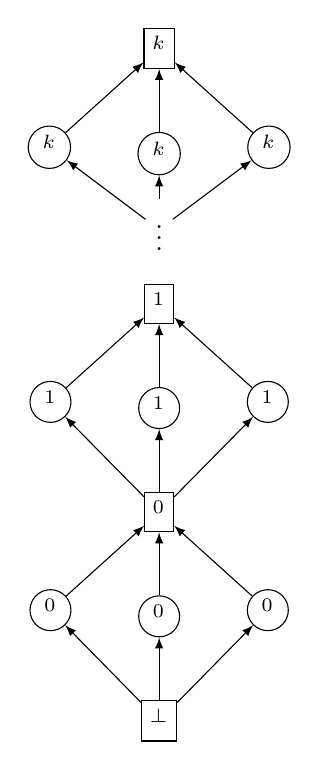
\begin{tikzpicture}[
    node distance=0.8cm and 1cm,
    base/.style={circle, draw, inner sep=2pt},
    any/.style={rectangle, draw, inner sep=3pt}
]
    % Grade k (Top)
    \node (anyk) [any] {$\Any^k$};
    \node (intk) [base, below left=of anyk] {$\Int^k$};
    \node (strk) [base, below=of anyk] {$\String^k$};
    \node (boolk) [base, below right=of anyk] {$\Bool^k$};
    
    \draw[-latex] (intk) -- (anyk);
    \draw[-latex] (strk) -- (anyk);
    \draw[-latex] (boolk) -- (anyk);

    % Ellipsis
    \node (vdots) [below=of strk, yshift=0.5cm] {\vdots};

    % Grade 1
    \node (any1) [any, below=of vdots, yshift=0.5cm] {$\Any^1$};
    \node (int1) [base, below left=of any1] {$\Int^1$};
    \node (str1) [base, below=of any1] {$\String^1$};
    \node (bool1) [base, below right=of any1] {$\Bool^1$};

    \draw[-latex] (int1) -- (any1);
    \draw[-latex] (str1) -- (any1);
    \draw[-latex] (bool1) -- (any1);
    
    % Connections from rank k-1 to k
    \path (vdots) edge[-latex] (intk);
    \path (vdots) edge[-latex] (strk);
    \path (vdots) edge[-latex] (boolk);

    % Grade 0
    \node (any0) [any, below=of str1] {$\Any^0$};
    \node (int0) [base, below left=of any0] {$\Int^0$};
    \node (str0) [base, below=of any0] {$\String^0$};
    \node (bool0) [base, below right=of any0] {$\Bool^0$};

    \draw[-latex] (int0) -- (any0);
    \draw[-latex] (str0) -- (any0);
    \draw[-latex] (bool0) -- (any0);
    
    % Connections from rank 0 to 1
    \draw[-latex] (any0) -- (int1);
    \draw[-latex] (any0) -- (str1);
    \draw[-latex] (any0) -- (bool1);
    
    \node (anybot) [any, below=of str0] {$\Any^{\bot}$};
    
    \draw[-latex] (anybot) -- (int0);
    \draw[-latex] (anybot) -- (str0);
    \draw[-latex] (anybot) -- (bool0);
\end{tikzpicture}
\caption[Hasse diagram of the graded type lattice]%
{Hasse diagram of the graded type lattice. Each rank $i$ consists of base types below $\Any^i$. 
The ranks are connected by the subtyping rule $\Any^i \le X^{i+1}$, forming a vertical chain.}
\label{fig:hassediagram}
\end{figure}

\section{The \textsf{Graded} Type System}
\label{sec:types}

We factor path-insensitivity at control-flow joins into a lightweight, \emph{grade}-annotated type algebra. Grades are \emph{static} metadata; runtime values are unannotated. Intuitively, a grade increases exactly when the analysis must \emph{commit to a base after imprecision}; i.e., when downcasting from $\Any$ to a concrete base via subtyping. Heterogeneous joins themselves do not raise the grade.

\paragraph{Indices and intuition.}
Grades range over $\mathbb{N}=\{0,1,2,\dots\}$, with two distinguished symbols:
a formal bottom $\bot$ used only by $\Any^{\bot}$, and an absorbing top $\infty$ used only by $\Any^{\infty}$.
Base literals appear at grade $0$.
We extend $\max$ by $\max(\bot,j)=j$ for $j\in\mathbb{N}$ (and never apply $+1$ to $\bot$ or $\infty$).

\begin{figure}[t]
\centering
\[
\begin{array}{rcll}
i &::=& 0 \mid 1 \mid 2 \mid \cdots & \text{(finite grades)}\\[2pt]
X &::=& \Int \mid \String \mid \Bool & \text{(base types)}\\[2pt]
\tau &::=& X^{i} \mid \Any^{i} \mid \Any^{\bot} \mid \Any^{\infty} & \text{(graded types)}
\end{array}
\]
\vspace{-2mm}
\caption{Syntax of graded types.}
\label{fig:syntax}
\end{figure}

\paragraph{Subtyping.}
Subtyping is the least reflexive–transitive relation generated by the rules in Fig.~\ref{fig:subtyping}. Intuitively, $\Any^{i}$ is the bottom of grade $i$; moving from grade $i$ to $i{+}1$ reflects a \emph{downcast assumption} to a concrete base; $\Any^{\infty}$ is an absorbing top; and $\Any^{\bot}$ seeds grade~$0$.

\begin{figure}[t]
\centering
\begin{mathpar}
\inferrule*[right=(grade)]
  { }
  { X^{i} \;\le\; \Any^{i} }\quad(i\in\mathbb{N})
\qquad
\inferrule*[right=(Step)]
  { }
  { \Any^{i} \;\le\; X^{i+1} }\quad(i\in\mathbb{N})
\end{mathpar}
\vspace{-3mm}
\caption{Generating rules for subtyping ($X\in\{\Int,\String,\Bool\}$).}
\label{fig:subtyping}
\end{figure}

\paragraph{Join (\texorpdfstring{$\sqcup$}{sqcup}).}
$\sqcup$ is the least upper bound w.r.t.\ $\le$.
Its definition proceeds by \emph{promotion to a common grade} followed by a same-grade join (Fig.~\ref{fig:join}).

\begin{figure}[t]
\centering
\textbf{Promotion to common grade.}
Define $\grade(\Any^{\bot}){=}\bot$, $\grade(\Any^{i}){=}i$, $\grade(X^{i}){=}i$, $\grade(\Any^{\infty}){=}\infty$.
For $\tau_1,\tau_2$ with finite grades or $\bot$, set $r=\max(\grade(\tau_1),\grade(\tau_2))$ and let
\[
\uparrow^{r}(\tau) \;=\;
\begin{cases}
\tau & \text{if } \grade(\tau)=r,\\
\Any^{r} & \text{if } \grade(\tau)<r\text{ (promote to least supertype at grade $r$).}
\end{cases}
\]
(If any operand is $\Any^{\infty}$, the join is $\Any^{\infty}$.)

\medskip
\textbf{Same-grade join (at grade $r\in\mathbb{N}$).}
For $X,Y\in\{\Int,\String,\Bool\}$ and $Z\in\{\Any,\Int,\String,\Bool\}$:
\[
\begin{array}{r@{\quad=\quad}l@{\qquad}l}
X^{r} \sqcup X^{r} & X^{r} & \text{(idempotence)}\\
X^{r} \sqcup Y^{r} & \Any^{r} & (X\neq Y)\ \text{(heterogeneous merge; no bump)}\\
\Any^{r} \sqcup Z^{r} & \Any^{r} & \text{(absorption)}\\
\end{array}
\]
\medskip
\textbf{Full definition.}
\[
\tau_1 \sqcup \tau_2 \;=\;
\begin{cases}
\Any^{\infty} & \text{if }\tau_1=\Any^{\infty}\text{ or }\tau_2=\Any^{\infty},\\
\uparrow^{r}(\tau_1)\ \sqcup\ \uparrow^{r}(\tau_2) & \text{where } r=\max(\grade(\tau_1),\grade(\tau_2)).
\end{cases}
\]
\vspace{-1mm}
\caption{Join: promote to a common grade, then same-grade join.}
\label{fig:join}
\end{figure}

\paragraph{Derived laws.}
For all $i\le j$ in $\mathbb{N}$ and $X\in\{\Int,\String,\Bool\}$:
\begin{align*}
&\textbf{Monotone grades:} && \Any^{i} \le \Any^{j},\quad X^{i} \le X^{j}.\\
&\textbf{Absorption (same grade):} && \Any^{i} \sqcup \tau^{i} = \Any^{i}.\\
&\textbf{Cross-grade absorption:} && \Any^{i} \sqcup \tau^{j} = \Any^{\max(i,j)}\quad(\text{with }\max(\bot,j)=j).\\
&\textbf{Heterogeneous same-grade merge:} && X^{i} \sqcup Y^{i}=\Any^{i}\ (X\neq Y).\\
&\textbf{Top absorption:} && \tau \sqcup \Any^{\infty}=\Any^{\infty}.\\
&\textbf{ACI of join:} && \text{$\sqcup$ is associative, commutative, idempotent.}
\end{align*}

\paragraph{Reading grades.}
With $\Any^{\bot}$ as a formal bottom, a finite grade $k\ge 0$ records the number of \emph{downcast assumptions} (steps of $\Any^{i}\le X^{i+1}$) witnessed so far along the abstract flow.
Once at $\Any^{k}$, further joins at grade $\le k$ do not escalate the grade; escalation requires a new downcast at or above grade $k$.
By convention, $\Any^{0}$ denotes imprecision \emph{without any forced assumption yet}:
merging heterogeneous bases at a join yields $\Any^{0}$ (after promotion), but grades increase only when a base is \emph{demanded} and a downcast $\Any^{i}\le X^{i+1}$ is taken.
Thus joins alone do not raise grades; uses that require a base do.

\medskip
This section defines only the graded type algebra.
The language and its abstract interpreter (expressions, statements, \textsf{while}) appear in the next section.

\paragraph*{Notation.}
We write $\Int,\String,\Bool,\Any$ in \textsf{sans} and use
$\grade(\cdot)$ and $\uparrow^{r}(\cdot)$ as defined above.
Include \texttt{mathpartir} for the inference rules.

\section{Language and Abstract Interpretation}
\label{sec:lang-ai}

We use a standard \textsf{while}-language with integers, strings, and booleans. Runtime semantics are conventional and unranked; ranks appear only in the abstract domain of \S\ref{sec:types}.

\subsection{Syntax and Concrete Semantics}

\begin{figure}[t]
\centering
\[
\begin{array}{rcll}
v &::=& n \in \mathbb{Z} \;\mid\; s \in \Sigma^* \;\mid\; \mathsf{true} \;\mid\; \mathsf{false} & \text{(values)}\\[1pt]
e &::=& v \;\mid\; x \;\mid\; e{+}e \;\mid\; \neg e \;\mid\; e \wedge e \;\mid\; e {=} e & \text{(expressions)}\\[1pt]
s &::=& \mathsf{skip} \;\mid\; x {:=} e \;\mid\; s; s \;\mid\; \mathsf{if}\; e\;\mathsf{then}\; s\;\mathsf{else}\; s \;\mid\; \mathsf{while}\; e\;\mathsf{do}\; s & \text{(statements)}
\end{array}
\]
\vspace{-2mm}
\caption{Syntax of the \textsf{while}-language.}
\label{fig:syntax-while}
\end{figure}

A \emph{state} is a total map $\sigma: \Var \to (\mathbb{Z}\cup\Sigma^*\cup\{\mathsf{true},\mathsf{false}\})$.
We write $\langle e,\sigma\rangle \Downarrow v$ for big-step expression evaluation and
$\langle s,\sigma\rangle \Downarrow \sigma'$ for statement evaluation. The rules are standard and deterministic:
(i) $x$ looks up $\sigma(x)$; (ii) $+$ denotes integer addition on integers and string concatenation on strings;
(iii) $\neg,\wedge$ operate on booleans; (iv) $=$ compares values for equality and yields a boolean; (v) assignments update the state; (vi) sequencing, conditional, and while follow the textbook rules, with $\mathsf{while}\;e\;\mathsf{do}\;s$ defined via the usual unrolling into an \textsf{if}.
We omit the routine rule schemata for space.

\subsection{Abstract Interpretation}

We interpret programs over the ranked type lattice of \S\ref{sec:types}.
An \emph{abstract environment} is a map $\Gamma:\Var\to\tau$.
Ordering and joins on environments are pointwise, using the subtyping $\le$ and join $\sqcup$ on types defined previously.

\paragraph{Rank-aware coercion to a base.}
For $X\in\{\Int,\String,\Bool\}$ and a type $\tau$, define the \emph{least $X$-supertype} (when it exists) by
\[
\ceil{\tau}_X \;=\; \min\nolimits_{\le}\,\{\,X^{k}\mid \tau \le X^{k}\,\}.
\]
Under the subtyping rules of Fig.~\ref{fig:subtyping}, $\ceil{\tau}_X$ always exists and is unique; intuitively, $\ceil{\cdot}_X$ “raises” $\tau$ to the nearest $X$-typed supertype, possibly increasing its rank.

\paragraph{Abstract expressions.}
We write $\Gamma \vdash e : \tau$ for abstract evaluation.

\begin{mathpar}
\inferrule*[right=(Lit)]
  { }
  { \Gamma \vdash n : \Int^{0} \qquad
    \Gamma \vdash s : \String^{0} \qquad
    \Gamma \vdash \mathsf{true} : \Bool^{0} \qquad
    \Gamma \vdash \mathsf{false} : \Bool^{0} }

\inferrule*[right=(Var)]
  { \Gamma(x)=\tau }
  { \Gamma \vdash x : \tau }

\inferrule*[right=(Sub)]
  { \Gamma \vdash e : \tau \quad \tau \le \tau' }
  { \Gamma \vdash e : \tau' }
\end{mathpar}

\noindent Binary and unary operators are typed by coercing operands to the relevant base(s) and then combining ranks via $max$; when multiple operator interpretations apply, we join their results:

\begin{mathpar}
\inferrule*[right=(Plus$_\Int$)]
  { \Gamma \vdash e_1:\tau_1 \quad \Gamma \vdash e_2:\tau_2 \\
    \ceil{\tau_1}_\Int = \Int^{i} \quad \ceil{\tau_2}_\Int = \Int^{j} }
  { \Gamma \vdash e_1{+}e_2 : \Int^{max(i,j)} }

\inferrule*[right=(Plus$_\String$)]
  { \Gamma \vdash e_1:\tau_1 \quad \Gamma \vdash e_2:\tau_2 \\
    \ceil{\tau_1}_\String = \String^{i} \quad \ceil{\tau_2}_\String = \String^{j} }
  { \Gamma \vdash e_1{+}e_2 : \String^{max(i,j)} }

\inferrule*[right=(Plus-Join)]
  { \Gamma \vdash e_1{+}e_2 : \tau_I \quad \Gamma \vdash e_1{+}e_2 : \tau_S }
  { \Gamma \vdash e_1{+}e_2 : \tau_I \sqcup \tau_S }
\end{mathpar}

\begin{mathpar}
\inferrule*[right=(Not)]
  { \Gamma \vdash e:\tau \quad \ceil{\tau}_\Bool=\Bool^{i} }
  { \Gamma \vdash \neg e : \Bool^{i} }
\qquad
\inferrule*[right=(And)]
  { \Gamma \vdash e_1:\tau_1 \quad \Gamma \vdash e_2:\tau_2 \\
    \ceil{\tau_1}_\Bool=\Bool^{i} \quad \ceil{\tau_2}_\Bool=\Bool^{j} }
  { \Gamma \vdash e_1 \wedge e_2 : \Bool^{max(i,j)} }
\end{mathpar}

\begin{mathpar}
\inferrule*[right=(Eq$_X$)]
  { X\in\{\Int,\String,\Bool\} \\
    \Gamma \vdash e_1:\tau_1 \quad \Gamma \vdash e_2:\tau_2 \\
    \ceil{\tau_1}_X = X^{i} \quad \ceil{\tau_2}_X = X^{j} }
  { \Gamma \vdash e_1 {=} e_2 : \Bool^{max(i,j)} }
\\
\inferrule*[right=(Eq-Join)]
  { \Gamma \vdash e_1{=}e_2 : \rho_1 \quad
    \Gamma \vdash e_1{=}e_2 : \rho_2 }
  { \Gamma \vdash e_1{=}e_2 : \rho_1 \sqcup \rho_2 }
\end{mathpar}

\paragraph{Abstract statements.}
We write $\Gamma \vdash s \triangleright \Gamma'$ for the abstract transformer.

\begin{mathpar}
\inferrule*[right=(Skip)]
  { }
  { \Gamma \vdash \mathsf{skip} \triangleright \Gamma }

\inferrule*[right=(Assign)]
  { \Gamma \vdash e : \tau }
  { \Gamma \vdash x {:=} e \triangleright \Gamma[x \mapsto \tau] }

\inferrule*[right=(Seq)]
  { \Gamma \vdash s_1 \triangleright \Gamma_1 \quad
    \Gamma_1 \vdash s_2 \triangleright \Gamma_2 }
  { \Gamma \vdash s_1; s_2 \triangleright \Gamma_2 }

\inferrule*[right=(If)]
  { \Gamma \vdash e : \tau \quad \ceil{\tau}_\Bool=\Bool^{i} \\
    \Gamma \vdash s_1 \triangleright \Gamma_1 \quad
    \Gamma \vdash s_2 \triangleright \Gamma_2 }
  { \Gamma \vdash \mathsf{if}\; e\;\mathsf{then}\; s_1\;\mathsf{else}\; s_2
      \triangleright (\Gamma_1 \sqcup \Gamma_2) }
\end{mathpar}

\noindent Loops are treated as least fixed points of a monotone functional (Kleene iteration suffices):

\begin{mathpar}
\inferrule*[right=(While)]
  { F(\Delta) \;=\; \Delta' \text{ where }
    \Delta \vdash e:\tau,\ \ceil{\tau}_\Bool=\Bool^{i},\ 
    \Delta \vdash s \triangleright \Delta' \\
    \Gamma^\star \text{ is the least solution of } \Gamma^\star = \Gamma \sqcup F(\Gamma^\star) }
  { \Gamma \vdash \mathsf{while}\; e\;\mathsf{do}\; s \triangleright \Gamma^\star }
\end{mathpar}

\paragraph{Remarks.}
All joins are those of \S\ref{sec:types} (promotion to a common rank followed by same-rank join).
Because programs have finitely many join sites and ranks only increase via such joins, the per-program abstract domain is finite up to the program’s control-flow structure; Kleene iteration therefore terminates without an additional widening.

\section{Properties}
\label{sec:properties}

We collect algebraic and metatheoretic facts about the ranked-type algebra of \S\ref{sec:types}
(with subtyping generated by \textsc{(rank)} $X^{i}\le \Any^{i}$ and \textsc{(Step)} $\Any^{i}\le X^{i+1}$ for $i\in\mathbb{N}$ and $X\in\{\Int,\String,\Bool\}$),
and about the abstract interpretation of \S\ref{sec:lang-ai}.
When proofs are immediate from the order structure, we group them.
Where nontrivial-but-straightforward, we sketch the argument.
Where false or currently unsettled, we say so.

\subsection{Order-theoretic facts (types and subtyping)}

\paragraph{Poset structure.}
\begin{itemize}
\item \textbf{Reflexivity and transitivity} of $\le$ hold by construction (least reflexive–transitive closure).
\item \textbf{Antisymmetry.} If $\tau_1\le \tau_2$ and $\tau_2\le \tau_1$ then $\tau_1=\tau_2$.
\emph{Sketch.} The generators are oriented “up”: within a rank ($X^{i}\to\Any^{i}$) or from rank $i$ to $i{+}1$ ($\Any^{i}\to X^{i+1}$). No generator points downward, so there are no nontrivial cycles.
\item \textbf{Infinite ascending chains (global).} The global order has $\cdots < X^{0} < \Any^{0} < X^{1} < \Any^{1} < \cdots$.
\end{itemize}

\paragraph{Join as LUB.}
The operator $\sqcup$ of \S\ref{sec:types} is defined as the \emph{least upper bound} w.r.t.\ $\le$.
\emph{Sketch.} Promotion to the common rank $r$ maps both arguments to least $r$-supertypes; the same-rank table then returns the least among their common $r$-supertypes (either a base $X^{r}$ when equal, or $\Any^{r}$ otherwise). Hence $\tau_1\sqcup\tau_2$ is the $\le$-LUB.

\paragraph{Basic algebraic laws.}
For all $i\le j$ and $X\in\{\Int,\String,\Bool\}$:
\[
\Any^{i}\le \Any^{j},\quad X^{i}\le X^{j},\qquad
\Any^{i}\sqcup \tau^{j}= \Any^{\max(i,j)},\qquad
X^{i}\sqcup Y^{i}=
\begin{cases}
X^{i} & (X=Y)\\
\Any^{i} & (X\neq Y)
\end{cases}
\]
Moreover, $\sqcup$ is associative, commutative, and idempotent (ACI).
All follow directly from the definition in Fig.~\ref{fig:join}.

\subsection{Typing meta-theory (core expressions)}

\paragraph{Decidability.}
Typing for expressions is decidable by structural recursion; subtyping checks are syntactic (the generated relation has a canonical decision procedure).

\paragraph{Principal types under least-rank discipline.}
If derivations always pick the \emph{least} admissible rank (no gratuitous subsumption), then every typable expression has a principal type unique up to $\le$.
Without this discipline, incomparable ranks may be derivable; principal typing may fail.

\paragraph{Canonical forms (bases).}
If $\vdash v:\Int^{i}$ then $v$ is an integer literal; similarly for $\String^{i}$ and $\Bool^{i}$.

\paragraph{Progress and preservation (expressions).}
For the core expression fragment, progress and preservation hold with ranks as annotations: if $\Gamma\vdash e:\tau$ and $e\to e'$ then $\Gamma\vdash e':\tau$.
(Operational rules are unchanged by ranks.)

\paragraph{No global safety theorem.}
The analysis is a may-analysis; it does not rule out runtime type errors for full programs. Ranks document precision loss; they do not enforce safety.

\subsection{Abstract interpretation: soundness, monotonicity, termination}

\paragraph{Monotonicity of transfer.}
All abstract expression and statement constructors are monotone in their inputs w.r.t.\ $\le$ (and pointwise on environments). In particular, $\ceil{\cdot}_X$ is monotone: $\tau\le\tau'$ implies $\ceil{\tau}_X \le \ceil{\tau'}_X$.

\paragraph{Soundness (may-analysis).}
Let $\alpha$ map concrete states to abstract environments by sending each concrete value to its base at rank $0$ and then closing upward under $\le$.
If $\alpha(\sigma)\le \Gamma$ and $\langle s,\sigma\rangle \Downarrow \sigma'$, and $\Gamma \vdash s \triangleright \Gamma'$, then $\alpha(\sigma') \le \Gamma'$.
\emph{Sketch.} By induction on the big-step derivation. Each operator coerces operands to the least base supertype via $\ceil{\cdot}_X$, which corresponds to taking an abstract upper bound; the join on environments is the LUB.

\paragraph{Termination.}
The global lattice has infinite height, so \emph{plain} Kleene iteration need not terminate in general (loops can propagate ever-increasing ranks via repeated downcasts on rising $\Any^{k}$).
We give two standard remedies; either suffices.

\smallskip
\noindent\emph{(A) Rank-capping widening.}
Fix a finite cap $K$ (e.g., number of distinct base-demand sites in the program).
Define a widening $\nabla_K$ pointwise on types by
\[
X^{i}\ \nabla_K\ X^{j} \;=\; X^{\min(\max(i,j),K)},\qquad
\Any^{i}\ \nabla_K\ \Any^{j} \;=\; \Any^{\min(\max(i,j),K)},
\]
and extend homomorphically to mixed pairs via promotion then capping. Then the standard iteration with $\sqcup$ and occasional $\nabla_K$ applications converges in finitely many steps to a post-fixpoint.

\smallskip
\noindent\emph{(B) Ghost-set product domain (per-program finiteness).}
Augment each variable’s abstract value with a finite set $R\subseteq J$ of \emph{site IDs} (base-demand and join sites).
Update $R$ by union at joins and add the current site at each downcast.
Interpret the rank as $|R|$ (or any monotone function of $R$).
Since $J$ is finite, the $R$-component has finite height; iteration terminates.
The numeric rank exposed to users can be $\min(|R|,K)$ for a chosen cap $K$.

\smallskip
Either approach preserves soundness; (B) additionally supports precise diagnostics (below).

\subsection{Diagnostics: bounded blame via ghost sets}

Instrument the analysis with ghost sets $R_x\subseteq J$ for each variable $x$ (where $J$ is the finite set of program sites that force a base after imprecision or merge flows).
At a join site $j$, set $R_x \leftarrow R_x^{\mathrm{then}}\cup R_x^{\mathrm{else}}\cup\{j\}$ pointwise.
At a downcast site $k$, set $R_x \leftarrow R_x\cup\{k\}$.
If a concrete run faults at a use of operands $\vec{e}$ at program point $p$, then some $j\in \bigcup R_{\vec{e}}(p)$ lies on the reaching-use history of a faulting operand.
Thus the number of candidate sites to inspect is bounded by $|\bigcup R_{\vec{e}}(p)|$.

\subsection{Optional top}
If $\Any^{\infty}$ is included, then trivially $\tau\le \Any^{\infty}$ and $\tau\sqcup \Any^{\infty}=\Any^{\infty}$ for all $\tau$.
All properties above remain valid.
Without $\Any^{\infty}$, there is no global top.

\subsection{What is unknown or intentionally left open}
\begin{itemize}
\item \textbf{Gradual guarantee (precision monotonicity).} \emph{Open.}
Ranks encode counts of assumptions; the usual gradual guarantee is formulated over a precision preorder and casts. A rank-indexed analogue remains to be stated and proved.
\item \textbf{Subject expansion (reverse preservation).} \emph{Generally false} in the presence of subtyping; we make no claim.
\item \textbf{Principal typings for full statements.} \emph{Open.} Fixed points and joins may admit incomparable environments unless a specific iteration schedule or widening is fixed.
\end{itemize}

\subsection{Summary}
$\langle\Types,\le,\sqcup\rangle$ forms a well-behaved join-semilattice; $\sqcup$ is the $\le$-LUB and ACI.
The abstract interpreter is monotone and sound as a may-analysis.
Termination requires either a simple rank-capping widening or a finite ghost-set product domain; both are standard and compatible with our diagnostics.
Ranks quantify analysis-time precision loss and support bounded-blame localization but do not constitute a safety guarantee.

\section{Illustrative Examples}
\label{sec:examples}

We illustrate abstract execution over the \emph{graded}-type lattice (types as in \S\ref{sec:types}).  
In each example we write abstract environments as
$\Gamma = \{\, x : \String^{0},\; b : \Bool^{0},\;\dots \,\}$
and update them pointwise. Joins and promotions follow \S\ref{sec:types}.
For loops, we assume the \emph{per-site idempotence} interpretation (ghost-set product): a downcast at a fixed program point raises the grade at most once.

\paragraph{Example 1 (literal assignment).}
\begin{quote}\ttfamily
x := 5
\end{quote}
Initial $\Gamma_0$ arbitrary.  
Typing $5:\Int^{0}$, assignment yields
\[
\Gamma_1 \;=\; \Gamma_0[\,x \mapsto \Int^{0}\,].
\]

\paragraph{Example 2 (simple heterogeneous branch).}
\begin{quote}\ttfamily
if b then x := 5 else x := "hi"
\end{quote}
Assume $\Gamma_0$ with $b:\Bool^{0}$.  
Then-branch gives $x:\Int^{0}$, else-branch gives $x:\String^{0}$.  
Same-grade heterogeneous join yields
\[
\Gamma_1 \;=\; \Gamma_0[\,x \mapsto \Any^{0}\,].
\]

\paragraph{Example 3 (correlated branches, safe at runtime).}
\begin{quote}\ttfamily
if b then x := 5 else x := "hello";\\
if b then x := x + 2 else x := x + "world"
\end{quote}
After the first \texttt{if}: $x:\Any^{0}$.  
Second \texttt{if}: each branch coerces $x$ to the needed base from grade $0$ (downcast to $X^{1}$),
computes $\Int^{1}$ or $\String^{1}$, and the branch join yields
\[
\Gamma_2 \;=\; \Gamma_0[\,x \mapsto \Any^{1}\,].
\]

\paragraph{Example 4 (swapped addends, unsafe at runtime; same abstract result).}
\begin{quote}\ttfamily
if b then x := 5 else x := "hello";\\
if b then x := x + "world" else x := x + 2
\end{quote}
Analysis identical to Example~3: after the first join $x:\Any^{0}$, each branch
locally coerces to the needed base (downcast to grade $1$), and the outer join gives
\[
\Gamma_2 \;=\; \Gamma_0[\,x \mapsto \Any^{1}\,].
\]

\paragraph{Example 5 (uniform loop).}
\begin{quote}\ttfamily
x := 0;\\
while c do x := x + 1
\end{quote}
$x:\Int^{0}$ after initialization; loop body preserves $\Int^{0}$;
fixed point at the loop head is $\Int^{0}$:
\[
\Gamma_{\!*} \;=\; \Gamma_0[\,x \mapsto \Int^{0}\,].
\]

\paragraph{Example 6 (heterogeneous loop).}
\begin{quote}\ttfamily
if b then x := 0 else x := "a";\\
while c do if d then x := x + 1 else x := x + "b"
\end{quote}
After the first \texttt{if}: $x:\Any^{0}$.  
Loop body: inner \texttt{if} coerces $x$ to $\Int^{1}$ or $\String^{1}$; same-grade join yields $\Any^{1}$.
With per-site idempotence, the loop head stabilizes at
\[
\Gamma_{\!*} \;=\; \Gamma_0[\,x \mapsto \Any^{1}\,].
\]

\paragraph{Example 7 (nested conditionals, one choke point but no use).}
\begin{quote}\ttfamily
if b then if c then x := 1 else x := "a"\\
\phantom{if b\ } else if d then x := "b" else x := 2
\end{quote}
Both sides of the outer \texttt{if} yield $x:\Any^{0}$; the outer join preserves that:
\[
\Gamma_1 \;=\; \Gamma_0[\,x \mapsto \Any^{0}\,].
\]

\paragraph{Example 8 (booleans and equality).}
\begin{quote}\ttfamily
x := (1 = 2);\\
y := ("a" = "a")
\end{quote}
Equality coerces both operands to the same base at grade $0$ and produces booleans at grade $0$:
\[
\Gamma_1 \;=\; \Gamma_0[\,x \mapsto \Bool^{0},\; y \mapsto \Bool^{0}\,].
\]

\paragraph{Example 9 (string concatenation).}
\begin{quote}\ttfamily
x := "a";\quad y := "b";\quad z := x + y
\end{quote}
Both operands are $\String^{0}$; result $\String^{0}$:
\[
\Gamma_1 \;=\; \Gamma_0[\,x \mapsto \String^{0},\;
                       y \mapsto \String^{0},\;
                       z \mapsto \String^{0}\,].
\]

\paragraph{Example 10 (mixing bases through a later join).}
\begin{quote}\ttfamily
if b then x := 1 else x := "a";\\
y := x;\\
if c then y := x else y := x
\end{quote}
After the first \texttt{if}: $x:\Any^{0}$.  
Copy $y:=x$ gives $y:\Any^{0}$.  
The final \texttt{if} does not change types (both branches identical);
overall
\[
\Gamma_1 \;=\; \Gamma_0[\,x \mapsto \Any^{0},\; y \mapsto \Any^{0}\,].
\]

\paragraph{Example 11 (guard typing is orthogonal).}
\begin{quote}\ttfamily
if (1 = 1) then x := "ok" else x := "ko"
\end{quote}
The guard yields $\Bool^{0}$; branches both give $\String^{0}$; join preserves $\String^{0}$:
\[
\Gamma_1 \;=\; \Gamma_0[\,x \mapsto \String^{0}\,].
\]

\paragraph{Example 12 (absorption with a precise base).}
\begin{quote}\ttfamily
if b then x := 1 else x := "a";\\
y := 0;\\
if c then x := x else x := y
\end{quote}
After the first \texttt{if}: $x:\Any^{0}$; and $y:\Int^{0}$.  
At the last \texttt{if}, joining $x:\Any^{0}$ with $y:\Int^{0}$ (promoted to $\Any^{0}$) leaves $x:\Any^{0}$.

\paragraph{Example 13 (disjoint effects on different variables).}
\begin{quote}\ttfamily
if b then x := 1 else x := "a";\quad
if c then y := true else y := false
\end{quote}
Final environment:
\[
\Gamma_1 \;=\; \Gamma_0[\,x \mapsto \Any^{0},\; y \mapsto \Bool^{0}\,].
\]

\paragraph{Example 14 (branch-local refinement, global imprecision).}
\begin{quote}\ttfamily
if b then x := 1 else x := "a";\\
if b then z := x + 2 else z := x + "b"
\end{quote}
Local coercions in each branch produce $\Int^{1}$ or $\String^{1}$ for $z$; the branch join yields $z:\Any^{1}$; $x$ remains $\Any^{0}$.

\paragraph{Example 15 (loop head as a choke point).}
\begin{quote}\ttfamily
x := 0;\\
while c do if d then x := x + 1 else x := x + 1
\end{quote}
Both inner branches agree ($\Int^{0}$); loop head join preserves $\Int^{0}$.

\paragraph{Example 16 (loop with branch-induced escalation).}
\begin{quote}\ttfamily
x := 0;\\
while c do if d then x := x + 1 else x := "b"
\end{quote}
Body joins (after needed coercion) to $\Any^{1}$; with per-site idempotence the loop head stabilizes at
\[
\Gamma_{\!*} \;=\; \Gamma_0[\,x \mapsto \Any^{1}\,].
\]

\paragraph{Example 17 (boolean loop).}
\begin{quote}\ttfamily
x := true;\\
while c do x := $\neg$ x
\end{quote}
Invariant $\Bool^{0}$; no grade change.

\paragraph{Example 18 (propagating imprecision through copy and use).}
\begin{quote}\ttfamily
if b then x := 1 else x := "a";\quad y := x;\\
z := (y = y)
\end{quote}
$x:\Any^{0}$, $y:\Any^{0}$.  
Equality coerces both operands to a common base from grade $0$ and yields $z:\Bool^{1}$.

\paragraph{Example 19 (multiple variables through one choke point).}
\begin{quote}\ttfamily
if b then \{ x := 1; y := "a" \} else \{ x := "b"; y := 2 \}
\end{quote}
Pointwise join yields $x:\Any^{0}$ and $y:\Any^{0}$.

\paragraph{Example 20 (no-op branches, no escalation).}
\begin{quote}\ttfamily
x := "a";\quad if b then x := x else x := x
\end{quote}
Both branches preserve $\String^{0}$; join preserves $\String^{0}$.

\section{Extensions}
\label{sec:extensions}

We sketch several conservative extensions of the core system. Each is named and can be adopted independently.

\subsection{\textsc{E1: Grade–Parametric Function Signatures \& Inference}}
\paragraph{Types.}
Augment types with (first–order) function arrows and grade quantification:
\[
\tau ::= \cdots \;\mid\; \tau \to \tau 
\qquad\qquad
\sigma ::= \forall \vec{i}.\ \tau
\]
where grade variables range over $\mathbb{N}$ and may appear in superscripts.
Typical shapes:
\[
\forall i.\ X^{i} \to X^{\,i+\alpha}
\qquad
\forall i,j.\ X^{i}\times Y^{j} \to Z^{\,\max(i,j)+\beta}
\]
with fixed nonnegative \emph{grade shifts} $\alpha,\beta \in \mathbb{N}$.

\paragraph{Examples.}
\begin{align*}
\textsf{id}_X &: \forall i.\ X^{i} \to X^{i} 
\\
\textsf{add1} &: \forall i.\ \textsf{Int}^{i} \to \textsf{Int}^{i}
\\
\textsf{concat\_a} &: \forall i.\ \textsf{String}^{i} \to \textsf{String}^{i}
\\
\textsf{downcast}_X &: \forall i.\ \textsf{Any}^{i} \to X^{\,i+1} \quad\text{(adds one grade)}
\\
\textsf{mix} &: \forall i,j.\ \textsf{Int}^{i}\times \textsf{String}^{j} \to \textsf{Any}^{\,\max(i,j)+1}
\end{align*}

\paragraph{Composition law.}
If $f:\forall i.\ X^{i}\!\to\! X^{\,i+\alpha}$ and $g:\forall i.\ X^{i}\!\to\! X^{\,i+\beta}$,
then $f\circ g:\forall i.\ X^{i}\!\to\! X^{\,i+\alpha+\beta}$.
For binary forms, grade shifts compose with $\max$ in the obvious way:
if $h:\forall i,j.\ X^{i}\times Y^{j}\to Z^{\,\max(i,j)+\gamma}$ and
$k:\forall i.\ Z^{i}\to Z^{\,i+\delta}$, then
$k\circ h:\forall i,j.\ X^{i}\times Y^{j}\to Z^{\,\max(i,j)+\gamma+\delta}$.

\paragraph{Typing (sketch).}
Application instantiates grade variables with concrete grades from the argument types,
then checks subtyping on bases and enforces the grade output equation given by the signature
(e.g., $i'\!=\!i{+}\alpha$, or $k'\!=\!\max(i,j){+}\beta$).

\paragraph{Inference.}
Associate unknown nonnegative shifts (e.g., $\alpha,\beta,\dots$) to function bodies and generate constraints from each use:
\[
r_{\text{out}} \;\ge\; r_{\text{in}} + \alpha
\qquad\text{or}\qquad
r_{\text{out}} \;\ge\; \max(r_1,r_2) + \beta
\]
together with base-type constraints.
Solve the resulting monotone system over $(\mathbb{N},\le)$ using least solutions
(e.g., Kleene iteration on $\max$/$+$ constraints); the \emph{principal} signature takes the least satisfying shifts.

\medskip

\subsection{\textsc{E2: Grades as Effects (Graded)}}
Treat “grade increase” as an effect grade.
A typing judgment carries a grade $g\in\mathbb{N}$; arrows become graded:
\(
\Gamma \vdash e : \tau \;!\; g
\)
and composition obeys $g$-addition while multi-argument operators use $g=\max$.
This yields a small-step algebra matching the grade equations in \textsc{E1}.

\subsection{\textsc{E3: Bounded–Grade Modes}}
Introduce a modal cap $\square_{\le k}$ that restricts programs (or interfaces) to yield grades $\le k$.
Useful for “precision budgets” and for rejecting overly imprecise code at module boundaries.

\subsection{\textsc{E4: Grade–Aware Cast Calculus}}
Add explicit casts $\langle \tau \Rightarrow \tau'\rangle e$ with types such as
$\forall i.\ \textsf{Any}^{i} \to X^{\,i+1}$,
and a runtime that either succeeds (raising grade by $+1$) or signals a checked failure.
This supports a \emph{bounded blame} story where failures are charged to specific cast sites.

\subsection{\textsc{E5: Shape–Preserving Joins for Data Types}}
Extend the lattice structurally:
\[
\textsf{List}\ X^{i} \;\sqcup\; \textsf{List}\ Y^{j}
\;=\; \textsf{List}\ \textsf{Any}^{\,\max(i,j)}
\]
(and analogously for products/sums), lifting the base rule into type constructors.

\subsection{\textsc{E6: SSA \& \texorpdfstring{$\phi$}{phi}–Site Instrumentation}}
In SSA, $\phi$–nodes are explicit choke points.
Label them with site IDs, propagate \emph{ghost culprit sets} alongside grades, and surface precise diagnostics:
“$x$ imprecise due to $\phi$ at blocks \#7,\#12”.

\subsection{\textsc{E7: Correlation Recovery (Selective Refinement)}}
Augment the analysis with lightweight relational facts (e.g., guard-sensitivity at chosen joins),
allowing post–join refinement that can \emph{lower} computed grades without changing the core lattice.

\subsection{\textsc{E8: Higher–Order Grade Polymorphism}}
Generalize \textsc{E1} to higher order:
\[
\textsf{map} : \forall i.\ (\textsf{Int}^{i}\!\to\!\textsf{Int}^{\,i+\alpha}) \to
(\textsf{List}\ \textsf{Int})^{i} \to (\textsf{List}\ \textsf{Int})^{\,i+\alpha}
\]
with inference propagating the shift $\alpha$ through higher-order uses.

\subsection{\textsc{E9: Interop with Gradual Typing}}
Keep our lattice (joins, grades) but add a consistency–based unknown $\star$ and casts.
Grade–aware casts (as in \textsc{E4}) could supply \emph{budgets} to a gradual system, while preserving our per–program convergence guarantees.

\subsection{\textsc{E10: Gradual Mode (Collapse \& Consistency)}}

\paragraph{Erasure.}
Define a collapse/erasure from graded to gradual types by
\[
\mathrm{erase}(\mathsf{Int}^{i})=\mathsf{Int},\quad
\mathrm{erase}(\mathsf{String}^{i})=\mathsf{String},\quad
\mathrm{erase}(\mathsf{Bool}^{i})=\mathsf{Bool},\quad
\mathrm{erase}(\mathsf{Any}^{i})=?,
\]
extended homomorphically over type constructors (products, sums, lists, \dots).

\paragraph{Consistency.}
On erased types, a standard consistency relation \(A \mathrel{\sim} B\) holds iff
(i) \(A=B\); or (ii) either side is \(?\); or (iii) type constructors match and components are pairwise consistent.
This is symmetric and shape-directed (not a subtyping order).

\paragraph{Casts and dynamics.}
Add explicit casts \(\langle \tau \Rightarrow \tau'\rangle e\).
Evaluation inserts runtime checks against the \emph{erased} target \(\mathrm{erase}(\tau')\);
failures raise \emph{blame} at the cast site.
The grade-aware downcast from \textsc{E4} is a typed form
\(\forall i.\ \mathsf{Any}^{i} \to X^{\,i+1}\);
the collapsed mode also admits ungraded casts by erasure.

\paragraph{Precision join correspondence.}
For base/shape-preserving cases,
\[
\mathrm{erase}(\tau_1 \sqcup \tau_2)
\;=\;
\mathrm{erase}(\tau_1)\ \sqcup_{\!\sim}\ \mathrm{erase}(\tau_2),
\]
where \(\sqcup_{\!\sim}\) is the usual precision join in gradual typing (e.g., \(\mathsf{Int}\sqcup_{\!\sim}\mathsf{String}=?\), and constructors lift \(?\) componentwise).

\paragraph{Obligations (left to future work).}
(i) \emph{Conservative extension}: erasure of a purely static program is well-typed in the gradual mode. 
(ii) \emph{Blame/coherence}: standard cast meta-theory over the erased core. 
(iii) \emph{Gradual guarantee}: precision monotonicity phrased on erased types. 
(iv) \emph{Embedding}: the graded system embeds into the gradual system by \(\mathrm{erase}\); the reverse picks finite-grade representatives.

\subsection{\textsc{E11: Metric Toggle — Downcast vs.\ Merge Counting}}

Our core uses the \emph{downcast-counting} metric:
heterogeneous same-grade joins return \(\Any^{r}\) (no bump), and grades increase only at subtyping steps \(\Any^{i}\le X^{\,i+1}\) when a base is demanded.
For completeness, we note an alternative \emph{merge-counting} variant and their relationship.

\paragraph{Downcast-counting (core).}
Subtyping generators:
\[
\inferrule*{ }{X^{i}\le \Any^{i}}
\qquad
\inferrule*{ }{\Any^{i}\le X^{\,i+1}}
\quad(i\in\mathbb{N},\ X\in\{\Int,\String,\Bool\})
\]
Join (analysis-time LUB w.r.t.\ \(\le\)): promote to common grade \(r\), then
\(X^{r}\sqcup Y^{r}=\Any^{r}\) for \(X\neq Y\), and \(\Any^{r}\) absorbs.

\paragraph{Merge-counting (alternative).}
Same subtyping as the core, but analysis join \emph{increments} on heterogeneous bases:
after promotion to grade \(r\), set \(X^{r}\sqcup Y^{r}=\Any^{\,r+1}\) for \(X\neq Y\).
Downcasts \(\Any^{i}\le X^{i}\) do not raise the grade in this variant.

\paragraph{Equivalence up to shift (informal).}
For straight-line code that immediately demands a base after each loss of correlation, both metrics produce the same grades up to a constant shift.
When imprecision is carried without commitment (values remain at \(\Any\) across joins), the metrics diverge:
merge-counting increments at the join; downcast-counting increments later, at the first demanded base.
Both variants preserve per-program finiteness and the bounded-blame story (culprit sets attach to, respectively, join sites vs.\ use sites).

\paragraph{Choosing a metric.}
Downcast-counting aligns grades with \emph{assumptions the analyzer had to make} at concrete use sites (casts/coercions);
merge-counting aligns grades with \emph{where correlation was lost} in control flow.
Either can be selected without changing the concrete semantics or the core lattice; only the analysis join and the intended diagnostic narrative differ.

\paragraph{Summary.}
\textsc{E1} makes grades first–class in function specifications with a simple, solvable constraint language.
\textsc{E2}–\textsc{E9} explore orthogonal axes—effects, budgets, casts, richer types, SSA integration, precision recovery, higher order, and interop—without disturbing the core algebra.

\section{Future Work}
\label{sec:future}

We outline directions that deepen the core while keeping it small. Each thread is orthogonal to the present design.

\subsection{Logical Readings (Curry--Howard)}
\paragraph{Graded unknowns as logical placeholders.}
Gradual typing admits a logic with an unknown proposition and a consistency relation. Our $\Any^{i}$ suggests a \emph{family} $\star^{i}$ annotated by a loss counter. A CH interpretation could attach evidence terms to discharge \emph{graded obligations} (casts-with-budgets) and prove a \emph{bounded-blame} theorem parameterized by grades/ghost sets. Open items: (i) a grade-indexed consistency/preorder; (ii) a grade-aware analogue of the gradual guarantee.

\paragraph{Subject expansion vs.\ diagnostic completeness.}
Reverse preservation fails with subtyping; a more realistic target is \emph{diagnostic completeness}: if a reduction gets stuck then some recorded culprit site is responsible. A proof-theoretic restatement would express this as locality of failed obligations.

\subsection{Resources and Quantitative Logics}
\paragraph{Ghost sets as permissions.}
Ghost culprit sets resemble quantitative resources. A grade-aware connective in a quantitative (idempotent) separation logic could enable modular bounds on the union of culprit sets. Unlike fractional permissions, our sets are idempotent: revisiting the same site does not increase the budget.

\paragraph{Cost models and budgets.}
Treat grades as an \emph{imprecision budget}. Explore grade-bounded modes (reject programs exceeding $k$) and synthesis/repair that minimizes maximal grade.

\subsection{Effects, Grades, and Indices}
\paragraph{Grades as effects.}
The mapping $X^{i}\mapsto X^{i+k}$ induced by a body behaves like a grade; multi-argument operators use $\max$. A semantics via graded monads/comonads or indexed effects could validate the $\max$/$+$ laws and composition.

\paragraph{Grade-parametric functions.}
We sketched types like $\forall i.\ \Int^i\!\to\!\Int^{i+3}$ and $\forall i,j.\ \Any^i\times\Bool^j\!\to\!\String^{\max(i,j)+1}$. Future work: formal typing/equational theory, principal-grade inference via lightweight $\max$/$+$ constraints, and interaction with polymorphism (generalization, ambiguity).

\paragraph{Guard optimization as static overload dispatch.}
Grade-parametric functions naturally induce a form of \emph{compile-time overloading} by grade: a function $f : \forall i.\ \tau^i \to \tau'^{i+k}$ can be specialized into distinct implementations $f_0, f_1, \ldots$ based on the input grade. 
Crucially, the grade-$0$ specialization $f_0 : \tau^0 \to \tau'^k$ operates on \emph{precisely-typed} values—those that have never passed through an imprecise join—and thus requires no runtime type guards or defensive checks.
Higher-grade specializations $f_j$ ($j > 0$) must account for potential imprecision and include appropriate dynamic checks.

This decomposition mirrors common JIT optimization strategies: hot paths with monomorphic types (corresponding to grade $0$) are compiled to tight, guard-free machine code, while polymorphic call sites (higher grades) retain full dynamic dispatch.
The grade annotation makes this optimization opportunity \emph{explicit} in the type system rather than relying on runtime profiling.
For instance, a list-processing function at grade $0$ knows all elements share the same concrete type and can vectorize operations or eliminate bounds checks, while the same function at grade $k > 0$ must remain defensive.
In effect, grades provide a static approximation of the runtime type stability that JIT compilers discover dynamically—enabling ahead-of-time optimization decisions based on the analysis-time precision guarantee.

\subsection{Semantic Foundations}
\paragraph{Abstract-interpretation account.}
A Galois-connection presentation would separate (i) the subtyping poset used for coercions and (ii) the analysis semilattice (promotion then same-grade LUB). This clarifies soundness from monotonicity and the role of promotion. For the \emph{merge-counting} variant (\S\ref{sec:extensions}), state precisely how the analysis join departs from the $\le$-LUB.

\paragraph{Domain theory with per-program slices.}
Globally the order has infinite height; per program the reachable slice is finite. A denotational model using compact/step-indexed elements could realize loop semantics as ordinary least fixed points while explaining per-program finiteness.

\subsection{Recovering Precision}
\paragraph{Correlation recovery.}
Integrate light relational domains (selected guard sensitivity, simple equalities) to \emph{lower} grades post hoc. A CEGAR-style loop: surface culprit sites, attempt focused refinement, iterate.

\paragraph{Shape-preserving joins.}
For sums/products/containers, develop uniform shape-lifting (e.g., $\List\,\Int^0 \sqcup \List\,\String^0 = \List\,\Any^{1}$) and study interaction with grade growth.

\subsection{Algorithmics and Tooling}
\paragraph{SSA $\phi$-sites.}
In SSA, $\phi$-nodes are explicit choke points. Label them with site IDs and propagate ghost sets to produce actionable diagnostics.

\paragraph{Inference and complexity.}
A least-grade subsumption discipline keeps expression typing deterministic. Analyze worst-case complexity under large join degrees, and engineer incremental fixed-point solvers; quantify bounds in terms of program size and number of base-demand sites.

\paragraph{User experience.}
Evaluate whether bounded-blame reports (e.g., ``$x$ imprecise due to sites \#7,\#12'') improve remediation compared to undifferentiated ``type is Any''.

\subsection{Relations to Gradual Typing}
Our lattice analysis remains distinct from consistency-based gradual typing. Two bridges: (i) a cast calculus with \emph{graded casts} (blame budgets); (ii) a \emph{conservative fragment} where grades never increase and the system coincides with a conventional static discipline. A grade-indexed gradual guarantee is open.

\subsection{Mechanization}
Mechanize (Coq/Agda/Isabelle): progress/preservation for the core expressions; monotonicity and convergence of the abstract interpreter (with cap/ghost product); and the bounded-blame lemma. A certified implementation can expose site IDs to the diagnostics layer.

\paragraph{Summary.}
Grades provide a compact, compositional handle on precision loss. Connecting them to resource logics, graded effects, and CH-style obligations looks feasible and promises principled diagnostics and stronger meta-theory without bloating the core.

\section{Related Work}
\label{sec:related}

\paragraph{Gradual typing and its foundations.}
Gradual typing provides a principled account of mixing static and dynamic typing \cite{SiekTaha2006}. Subsequent work articulated meta-theoretic criteria such as the \emph{Gradual Guarantee} and precision monotonicity \cite{SiekGarciaTaha2015}. \emph{Abstracting Gradual Typing (AGT)} recasts gradual typing via abstract interpretation, formulating a Galois connection between precise and gradual types and deriving typing and casts from abstraction/concretization \cite{GarciaClarkTanter2016}. More recently, \emph{Gradual Type Theory} axiomatizes casts, the dynamic type, and the gradual guarantee in a type-theoretic setting, supplying logical tools to reason about equivalence and optimization \cite{NewLicataAhmed2021}. Our proposal is deliberately cast-free and purely static: instead of a single collapsed unknown, we expose an \emph{unfolded} family (grades) that measures analysis imprecision without altering operational semantics.

\paragraph{AGT versus unfolded unknowns.}
AGT uses a \emph{single} unknown ($?$) whose meaning is given by concretization to a set of precise types; consistency and casts are derived systematically from the abstraction. In our system, there is a \emph{countable family} $\Any^{0},\Any^{1},\ldots$ indexing \emph{assumption depth} in a purely static abstract domain: same-grade joins are conservative LUBs, and grades increase only at base-demand sites (downcasts). There is a simple erasure map $\mathrm{erase}(X^{i})=X$ and $\mathrm{erase}(\Any^{i})=?$ that embeds our types into AGT’s gradual types; conversely, all $\Any^{i}$ lie over the same AGT unknown, so grades add provenance information orthogonal to AGT’s precision preorder. Thus our system can be viewed as an \emph{unfolded} static stratum of AGT (no runtime casts), with grades recording where/how many assumptions were forced.

\paragraph{Gradual effect and annotation systems.}
Generalizations beyond simple types include gradual type-and-effect systems \cite{BanadosSchwerterGarciaTanter2016} and frameworks for gradualizing annotated type systems \cite{ThiemannFennell2014}. These quantify imprecision via a \emph{single} unknown element ($?$) and a consistency relation. In contrast, our grades stratify imprecision arithmetically, recording how many assumptions were needed, while retaining a conventional join-semilattice discipline.

\paragraph{Blame calculi and static blame.}
The blame calculus connects gradual/hybrid typing with higher-order contracts and proves the blame theorem: when casts fail, responsibility lies on the less-precisely typed side \cite{WadlerFindler2009}; polymorphic extensions preserve these guarantees \cite{AhmedFindlerSiekWadler2011}. More recently, \emph{static blame} predicts potential blame without executing programs \cite{SuCulpepper2024}. Our setting shares the diagnostic spirit but introduces neither casts nor contract boundaries; the grade is a static, flow-sensitive measure of precision loss at control-flow joins and later downcasts.

\paragraph{Soft and quasi-static typing.}
Soft typing \cite{CartwrightFagan1991} and quasi-static typing \cite{Thatte1990} prefigure many aims of gradual typing: inferring permissive types and inserting checks as needed (often around a greatest element such as $\Omega$ or \textsf{Dyn}). By contrast, our analysis remains fully static and is not a source-to-source transformation; quantitative information is recorded as a grade in the abstract domain rather than materialized as runtime checks.

\paragraph{Typed/untyped interoperation via ``like'' types.}
Thorn’s \emph{like types} enable fine-grained interoperation between typed and untyped code while retaining optimization potential in typed regions \cite{WrigstadEtAl2010}. This is complementary: it proposes language constructs and runtime checks for interoperability, whereas we supply a static accounting of precision loss that can inform where such boundaries matter.

\paragraph{Abstract interpretation.}
Methodologically, our analysis is a standard monotone, flow-sensitive abstract interpretation \cite{CousotCousot1977}. The novelty lies in the abstract domain: an \emph{unfolded} per-program slice in which the conservative same-grade join is the LUB and grade increases only at finitely many base-demand sites (idempotent per site). Thus fixed points exist without bespoke widenings, and the diagnostic information (grades and culprit sites) is exposed rather than collapsed.

\paragraph{Path sensitivity and disjunctive completion.}
Precision at joins can be recovered by duplicating control-flow contexts rather than collapsing them: 
trace partitioning, disjunctive completion, and configurable program analysis (CPA) are standard ways to pay for path sensitivity where it matters \cite{MauborgneRival2005,BeyerHenzinger2007}.
Our approach is orthogonal: we remain path-insensitive but \emph{quantify} and \emph{attribute} the assumptions forced by later uses.
Rather than keeping disjunctions, we collapse early and carry a small integral signal (\emph{grade}) plus culprit sites; this keeps fixed-point iteration cheap while producing actionable diagnostics.

\paragraph{Flow/occurrence typing and control-flow refinement.}
Occurrence typing as in Typed Racket refines variable types across branches and joins by inspecting guards, recovering precision without runtime checks \cite{TobinHochstadtFelleisen2008}.
Industrial analyzers (e.g., TypeScript, Flow) employ related control-flow analysis with unions.
These systems aim to \emph{avoid} imprecision; our aim is to \emph{make residual imprecision explicit and localizable}.
Where occurrence typing succeeds, our grades stay low; when correlations are untracked (by design), grades expose how many use-site assumptions were needed and where they arose.

\section{Conclusion}
\label{sec:conclusion}

We introduced a small, compositional static analysis that makes path-insensitive precision loss explicit via a ranked algebra of types. Base types and $\Any$ carry a nonnegative rank; same-rank heterogeneous joins are conservative, and ranks increase only when the analysis commits to a base after imprecision ($\Any^{i}\!\le\!X^{\,i+1}$). We instantiated this domain in a standard abstract interpreter for a \textsf{while}-language, proved monotonicity and soundness (as a may-analysis), and explained termination either by a simple rank-capping widening or by a finite ghost-set product domain. The rank and its associated culprit-set provide actionable diagnostics: they localize where assumptions were forced and bound how much imprecision a value carries.

The approach is deliberately cast-free and leaves operational semantics unchanged. It relates cleanly to gradual typing: collapsing ranks and adding consistency/casts recovers a conventional gradual system, while retaining the ranked domain yields an ``unfolded'' static account of imprecision provenance. Extensions—rank-parametric function signatures, rank-as-effect grades, shape-preserving joins, SSA $\phi$-site instrumentation, and a gradual mode—fit without disturbing the core algebra.

Limitations are clear: the analysis is path-insensitive, does not guarantee absence of runtime type errors, and we have not attempted an empirical evaluation here. The \S\ref{sec:future} agenda outlines next steps (graded semantics, precision recovery, mechanization). The core contribution is a minimal algebra and analysis that expose, rather than collapse, the structure of precision loss—yielding principled and explainable static diagnostics.


%\newpage
\bibliographystyle{plain}
\bibliography{references}

\end{document}
